\documentclass[aspectratio=169]{beamer}

\makeatletter
\def\input@path{{../BeamerTemplate/theme/}}
\makeatother

\usepackage[utf8]{inputenc}
\usepackage{lmodern}
\usepackage[T1]{fontenc}
\usepackage{listings}
\usepackage{tikz}
\usetikzlibrary{arrows.meta, positioning, shapes.geometric, calc, shapes.multipart, matrix, trees}

\usetheme{CleanEasy}
\input{../BeamerTemplate/configs/configs}

\title{Segment Trees}
\subtitle{Data Structures}
\author{Minseok Jeon}
\institute{DGIST}
\date{\today}

\begin{document}

\begin{frame}
  \titlepage
\end{frame}

\begin{frame}{Table of Contents}
  \tableofcontents
\end{frame}

\section{Introduction to Segment Trees}

\begin{frame}{What is a Segment Tree?}
  \textbf{Segment Tree:} A binary tree structure for efficient range queries and updates

  \vspace{0.5cm}
  \textbf{Key Properties:}
  \begin{itemize}
    \item Each node represents an interval/segment of the array
    \item Leaf nodes represent single elements
    \item Internal nodes store aggregate information about their range
    \item Height: O(log n) for n elements
  \end{itemize}

  \vspace{0.5cm}
  \textbf{Common Operations:}
  \begin{itemize}
    \item Range sum/min/max queries
    \item Point updates
    \item Range updates (with lazy propagation)
  \end{itemize}

  \vspace{0.3cm}
  \textbf{Time Complexity:} O(log n) for queries and updates
\end{frame}

\begin{frame}{Motivation}
  \textbf{Problem:} Given array, answer multiple queries:
  \begin{itemize}
    \item What is the sum of elements from index $i$ to $j$?
    \item Update element at index $k$
  \end{itemize}

  \vspace{0.5cm}
  \textbf{Naive Approach:}
  \begin{itemize}
    \item Query: O(n) - iterate through range
    \item Update: O(1) - change single element
  \end{itemize}

  \vspace{0.5cm}
  \textbf{Prefix Sum Approach:}
  \begin{itemize}
    \item Query: O(1) - prefix[j] - prefix[i-1]
    \item Update: O(n) - rebuild prefix array
  \end{itemize}

  \vspace{0.5cm}
  \textbf{Segment Tree Solution:}
  \begin{itemize}
    \item Query: O(log n) - traverse tree
    \item Update: O(log n) - update path to root
    \item Best of both worlds!
  \end{itemize}
\end{frame}

\begin{frame}{Applications}
  Segment trees are versatile and widely used:

  \vspace{0.3cm}
  \begin{enumerate}
    \item \textbf{Competitive Programming:}
      \begin{itemize}
        \item Range sum/min/max queries with updates
        \item Finding k-th smallest element in range
        \item Maximum subarray sum in range
      \end{itemize}
    \item \textbf{Databases:}
      \begin{itemize}
        \item Range aggregation queries
        \item Time-series databases
        \item Spatial indexes
      \end{itemize}
    \item \textbf{Graphics \& Games:}
      \begin{itemize}
        \item Rectangle union area
        \item Collision detection
        \item Visibility queries
      \end{itemize}
    \item \textbf{Other:}
      \begin{itemize}
        \item Network monitoring
        \item Financial OHLC queries
        \item Computational geometry
      \end{itemize}
  \end{enumerate}
\end{frame}

\section{Building Segment Trees}

\begin{frame}{Tree Structure}
  \textbf{Array:} [1, 3, 5, 7, 9, 11]

  \begin{center}
    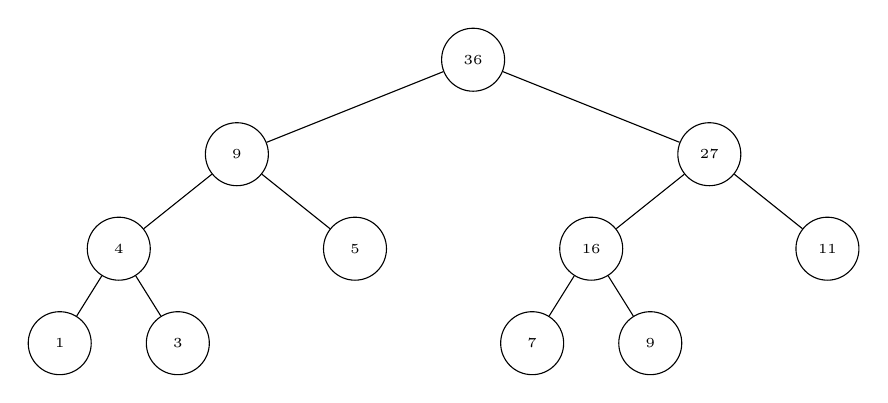
\begin{tikzpicture}[
      level distance=1.2cm,
      level 1/.style={sibling distance=6cm},
      level 2/.style={sibling distance=3cm},
      level 3/.style={sibling distance=1.5cm},
      every node/.style={circle, draw, minimum size=0.8cm, font=\tiny}
    ]
      \node {36}
        child {node {9}
          child {node {4}
            child {node {1}}
            child {node {3}}
          }
          child {node {5}}
        }
        child {node {27}
          child {node {16}
            child {node {7}}
            child {node {9}}
          }
          child {node {11}}
        };
    \end{tikzpicture}
  \end{center}

  \vspace{0.3cm}
  \small
  Each node stores: \textbf{sum} of its range
\end{frame}

\begin{frame}{Array Representation}
  \textbf{Tree stored in array:} Similar to heap representation

  \vspace{0.3cm}
  \textbf{Index mapping:}
  \begin{itemize}
    \item Node at index $i$ has children at $2i$ and $2i+1$
    \item Parent of node $i$ is at $i/2$
    \item Root at index 1
  \end{itemize}

  \vspace{0.5cm}
  \textbf{Space requirement:}
  \begin{itemize}
    \item For array of size $n$, need $\approx 4n$ space
    \item Height = $\lceil \log_2 n \rceil$
    \item Total nodes = $2^{h+1} - 1 < 4n$
  \end{itemize}

  \vspace{0.5cm}
  \textbf{Array layout for [1, 3, 5, 7, 9, 11]:}
  \begin{center}
    \small
    \begin{tabular}{|c|c|c|c|c|c|c|c|c|c|c|c|c|}
      \hline
      Index & 1 & 2 & 3 & 4 & 5 & 6 & 7 & 8 & 9 & 12 & 13 \\
      \hline
      Value & 36 & 9 & 27 & 4 & 5 & 16 & 11 & 1 & 3 & 7 & 9 \\
      \hline
    \end{tabular}
  \end{center}
\end{frame}

\begin{frame}[fragile]{Building the Tree - Recursive}
  \begin{lstlisting}[language=Python, basicstyle=\ttfamily\footnotesize]
class SegmentTree:
    def __init__(self, arr):
        self.n = len(arr)
        self.tree = [0] * (4 * self.n)
        self.arr = arr
        if self.n > 0:
            self.build(1, 0, self.n - 1)

    def build(self, node, start, end):
        """
        Build segment tree recursively
        node: current node index in tree array
        [start, end]: range this node represents
        """
        if start == end:
            # Leaf node - copy array element
            self.tree[node] = self.arr[start]
            return

        mid = (start + end) // 2
        left_child = 2 * node
        right_child = 2 * node + 1

        # Build left and right subtrees
        self.build(left_child, start, mid)
        self.build(right_child, mid + 1, end)

        # Internal node stores sum of children
        self.tree[node] = self.tree[left_child] + self.tree[right_child]
  \end{lstlisting}
\end{frame}

\begin{frame}[fragile]{Building the Tree - Iterative}
  \textbf{More efficient approach using 2n space:}

  \begin{lstlisting}[language=Python, basicstyle=\ttfamily\footnotesize]
def build_iterative(arr):
    """Build segment tree iteratively - more efficient"""
    n = len(arr)
    tree = [0] * (2 * n)

    # Copy array to second half
    for i in range(n):
        tree[n + i] = arr[i]

    # Build tree by calculating parents
    for i in range(n - 1, 0, -1):
        tree[i] = tree[2 * i] + tree[2 * i + 1]

    return tree
  \end{lstlisting}

  \vspace{0.5cm}
  \textbf{Advantages:}
  \begin{itemize}
    \item Uses only 2n space (vs 4n for recursive)
    \item Simpler index calculations
    \item No recursion overhead
  \end{itemize}

  \vspace{0.3cm}
  \textbf{Time Complexity:} O(n) for both approaches
\end{frame}

\section{Range Queries}

\begin{frame}{Query Types}
  Segment trees support various aggregate queries:

  \vspace{0.5cm}
  \textbf{1. Range Sum:}
  \begin{itemize}
    \item Query: sum(left, right) = sum of elements in [left, right]
    \item Combine: $\text{sum}_{\text{left}} + \text{sum}_{\text{right}}$
  \end{itemize}

  \vspace{0.3cm}
  \textbf{2. Range Minimum:}
  \begin{itemize}
    \item Query: min(left, right) = minimum element in [left, right]
    \item Combine: $\min(\text{min}_{\text{left}}, \text{min}_{\text{right}})$
  \end{itemize}

  \vspace{0.3cm}
  \textbf{3. Range Maximum:}
  \begin{itemize}
    \item Query: max(left, right) = maximum element in [left, right]
    \item Combine: $\max(\text{max}_{\text{left}}, \text{max}_{\text{right}})$
  \end{itemize}

  \vspace{0.3cm}
  \textbf{4. Other Operations:}
  \begin{itemize}
    \item GCD of range
    \item XOR of range
    \item Any associative operation!
  \end{itemize}
\end{frame}

\begin{frame}[fragile]{Range Sum Query Implementation}
  \begin{lstlisting}[language=Python, basicstyle=\ttfamily\footnotesize]
def query_sum(self, node, start, end, left, right):
    """
    Query sum in range [left, right]
    node: current node
    [start, end]: range of current node
    [left, right]: query range
    """
    # Case 1: No overlap
    if right < start or left > end:
        return 0

    # Case 2: Complete overlap
    if left <= start and end <= right:
        return self.tree[node]

    # Case 3: Partial overlap
    mid = (start + end) // 2
    left_sum = self.query_sum(2 * node, start, mid, left, right)
    right_sum = self.query_sum(2 * node + 1, mid + 1, end,
                                left, right)

    return left_sum + right_sum

# Wrapper method
def range_sum(self, left, right):
    return self.query_sum(1, 0, self.n - 1, left, right)
  \end{lstlisting}
\end{frame}

\begin{frame}{Query Visualization}
  \textbf{Query: sum(2, 4) in array [1, 3, 5, 7, 9, 11]}

  \begin{center}
    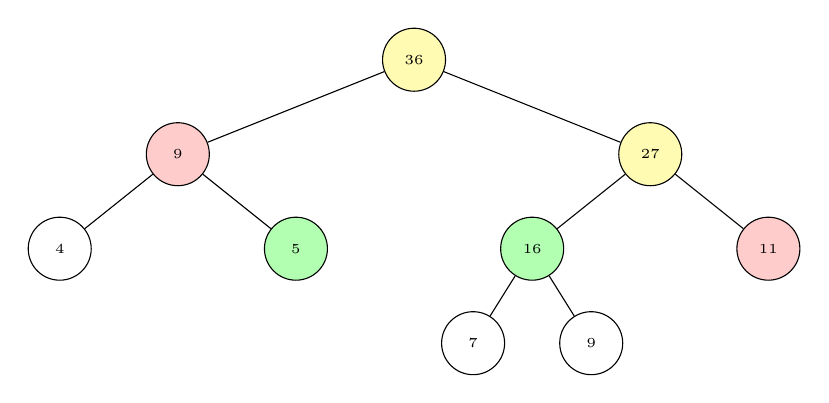
\begin{tikzpicture}[
      level distance=1.2cm,
      level 1/.style={sibling distance=6cm},
      level 2/.style={sibling distance=3cm},
      level 3/.style={sibling distance=1.5cm},
      every node/.style={circle, draw, minimum size=0.8cm, font=\tiny}
    ]
      \node[fill=yellow!30] {36}
        child {node[fill=red!20] {9}
          child {node {4}}
          child {node[fill=green!30] {5}}
        }
        child {node[fill=yellow!30] {27}
          child {node[fill=green!30] {16}
            child {node {7}}
            child {node {9}}
          }
          child {node[fill=red!20] {11}}
        };
    \end{tikzpicture}
  \end{center}

  \vspace{0.3cm}
  \small
  \textcolor{green!70!black}{Green: Complete overlap} \quad
  \textcolor{yellow!70!black}{Yellow: Partial overlap} \quad
  \textcolor{red!70!black}{Red: No overlap}

  \vspace{0.3cm}
  Result: 5 + 16 = 21 (which equals 5 + 7 + 9 \checkmark)
\end{frame}

\begin{frame}[fragile]{Range Minimum Query}
  \textbf{Similar structure, different combine operation:}

  \begin{lstlisting}[language=Python, basicstyle=\ttfamily\footnotesize]
class SegmentTreeMin:
    def __init__(self, arr):
        self.n = len(arr)
        self.tree = [float('inf')] * (4 * self.n)
        self.arr = arr
        if self.n > 0:
            self.build(1, 0, self.n - 1)

    def build(self, node, start, end):
        if start == end:
            self.tree[node] = self.arr[start]
            return

        mid = (start + end) // 2
        self.build(2 * node, start, mid)
        self.build(2 * node + 1, mid + 1, end)

        # Store minimum of children
        self.tree[node] = min(self.tree[2 * node],
                             self.tree[2 * node + 1])

    def query_min(self, node, start, end, left, right):
        if right < start or left > end:
            return float('inf')  # Identity for min

        if left <= start and end <= right:
            return self.tree[node]

        mid = (start + end) // 2
        return min(self.query_min(2*node, start, mid, left, right),
                   self.query_min(2*node+1, mid+1, end, left, right))
  \end{lstlisting}
\end{frame}

\begin{frame}{Query Time Complexity}
  \textbf{Why is query O(log n)?}

  \vspace{0.5cm}
  \textbf{Analysis:}
  \begin{itemize}
    \item Tree height: $h = \lceil \log_2 n \rceil$
    \item At each level, visit at most 2 nodes
    \item Total nodes visited: $\leq 2h = O(\log n)$
  \end{itemize}

  \vspace{0.5cm}
  \textbf{Why at most 2 nodes per level?}
  \begin{enumerate}
    \item Start at root
    \item At each level, query range can intersect at most 2 children
    \item Left boundary intersects one child
    \item Right boundary intersects another child
    \item Middle parts are completely covered (return immediately)
  \end{enumerate}

  \vspace{0.5cm}
  \textbf{Best case:} O(1) - complete overlap at root\\
  \textbf{Worst case:} O(log n) - query single element\\
  \textbf{Average case:} O(log n)
\end{frame}

\section{Point Updates}

\begin{frame}[fragile]{Point Update Implementation}
  \begin{lstlisting}[language=Python, basicstyle=\ttfamily\footnotesize]
def update_point(self, node, start, end, idx, value):
    """
    Update element at index idx to value
    """
    if start == end:
        # Leaf node - update value
        self.arr[idx] = value
        self.tree[node] = value
        return

    mid = (start + end) // 2

    if idx <= mid:
        # Update in left subtree
        self.update_point(2 * node, start, mid, idx, value)
    else:
        # Update in right subtree
        self.update_point(2 * node + 1, mid + 1, end, idx, value)

    # Update current node from children
    self.tree[node] = (self.tree[2 * node] +
                       self.tree[2 * node + 1])

# Wrapper method
def update(self, idx, value):
    self.update_point(1, 0, self.n - 1, idx, value)
  \end{lstlisting}
\end{frame}

\begin{frame}{Update Visualization}
  \textbf{Update index 2 from 5 to 8 (delta = +3)}

  \vspace{0.3cm}
  \textbf{Before:}
  \begin{center}
    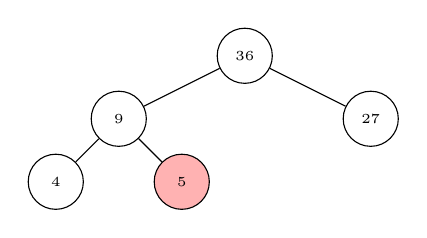
\begin{tikzpicture}[
      level distance=1cm,
      level 1/.style={sibling distance=4cm},
      level 2/.style={sibling distance=2cm},
      every node/.style={circle, draw, minimum size=0.7cm, font=\tiny},
      scale=0.8
    ]
      \node {36}
        child {node {9}
          child {node {4}}
          child {node[fill=red!30] {5}}
        }
        child {node {27}};
    \end{tikzpicture}
  \end{center}

  \vspace{0.3cm}
  \textbf{After:}
  \begin{center}
    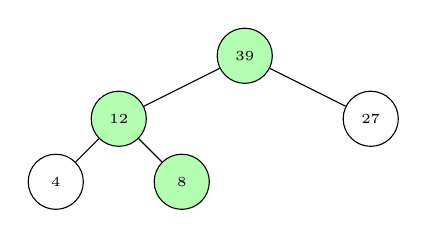
\begin{tikzpicture}[
      level distance=1cm,
      level 1/.style={sibling distance=4cm},
      level 2/.style={sibling distance=2cm},
      every node/.style={circle, draw, minimum size=0.7cm, font=\tiny},
      scale=0.8
    ]
      \node[fill=green!30] {39}
        child {node[fill=green!30] {12}
          child {node {4}}
          child {node[fill=green!30] {8}}
        }
        child {node {27}};
    \end{tikzpicture}
  \end{center}

  \vspace{0.3cm}
  \small
  Updated nodes: [2], [0-2], [0-5] - Only O(log n) nodes!
\end{frame}

\begin{frame}{Update Time Complexity}
  \textbf{Why is update O(log n)?}

  \vspace{0.5cm}
  \textbf{Path from leaf to root:}
  \begin{itemize}
    \item Update travels from leaf to root
    \item Path length = tree height = $\lceil \log_2 n \rceil$
    \item Each ancestor needs updating
  \end{itemize}

  \vspace{0.5cm}
  \textbf{Example for n = 8:}
  \begin{itemize}
    \item Height = 3
    \item Update path: leaf $\rightarrow$ parent $\rightarrow$ grandparent $\rightarrow$ root
    \item 4 nodes total = $\log_2 8 + 1$
  \end{itemize}

  \vspace{0.5cm}
  \textbf{Comparison:}
  \begin{itemize}
    \item Naive array: O(1) update, but O(n) query
    \item Prefix sum: O(n) update (rebuild), O(1) query
    \item Segment tree: O(log n) update, O(log n) query \checkmark
  \end{itemize}
\end{frame}

\section{Range Updates with Lazy Propagation}

\begin{frame}{The Range Update Problem}
  \textbf{Problem:} Add delta to all elements in range [left, right]

  \vspace{0.5cm}
  \textbf{Naive approach:}
%   \begin{lstlisting}[language=Python, basicstyle=\ttfamily\footnotesize]
% def update_range_naive(self, left, right, delta):
%     for i in range(left, right + 1):
%         self.update(i, self.arr[i] + delta)
%   \end{lstlisting}

  \textbf{Time:} O(n log n) - Too slow!

  \vspace{0.5cm}
  \textbf{Problem:}
  \begin{itemize}
    \item Range size can be O(n)
    \item Each update is O(log n)
    \item Total: O(n log n)
  \end{itemize}

  \vspace{0.5cm}
  \textbf{Solution: Lazy Propagation}
  \begin{itemize}
    \item Mark nodes as "lazy" instead of updating immediately
    \item Defer updates until actually needed
    \item Push lazy values down only when queried
    \item Achieves O(log n) range update!
  \end{itemize}
\end{frame}

\begin{frame}{Lazy Propagation Concept}
  \textbf{Key Idea:} Don't update eagerly, be lazy!

  \vspace{0.5cm}
  \textbf{Lazy Array:}
  \begin{itemize}
    \item Additional array: \texttt{lazy[]} same size as tree
    \item \texttt{lazy[node]} = pending update for this node's range
    \item When \texttt{lazy[node] $\neq$ 0}: node needs update
  \end{itemize}

  \vspace{0.5cm}
  \textbf{Update Strategy:}
  \begin{enumerate}
    \item Find nodes completely covered by update range
    \item Mark them as lazy (don't go deeper!)
    \item Push lazy values down only when needed:
      \begin{itemize}
        \item During next query
        \item During next update that overlaps
      \end{itemize}
  \end{enumerate}

  \vspace{0.5cm}
  \textbf{Benefits:}
  \begin{itemize}
    \item Range update: O(log n) instead of O(n log n)
    \item Multiple updates before query: Very efficient
    \item Updates batched and propagated lazily
  \end{itemize}
\end{frame}

\begin{frame}[fragile]{Push Down Operation}
  \begin{lstlisting}[language=Python, basicstyle=\ttfamily\footnotesize]
def push_down(self, node, start, end):
    """Propagate lazy value to children"""
    if self.lazy[node] != 0:
        # Apply lazy value to current node
        range_size = end - start + 1
        self.tree[node] += range_size * self.lazy[node]

        # If not leaf, propagate to children
        if start != end:
            self.lazy[2 * node] += self.lazy[node]
            self.lazy[2 * node + 1] += self.lazy[node]

        # Clear lazy value
        self.lazy[node] = 0
  \end{lstlisting}

  \vspace{0.3cm}
  \textbf{Key Points:}
  \begin{itemize}
    \item Apply lazy value to current node
    \item Pass lazy value to children (don't apply recursively!)
    \item Clear current node's lazy value
    \item Call before any operation on a node
  \end{itemize}
\end{frame}

\begin{frame}[fragile]{Range Update with Lazy}
  \begin{lstlisting}[language=Python, basicstyle=\ttfamily\tiny]
def update_range(self, node, start, end, left, right, delta):
    """Add delta to range [left, right]"""
    # Push down pending updates first
    self.push_down(node, start, end)

    # No overlap
    if right < start or left > end:
        return

    # Complete overlap
    if left <= start and end <= right:
        # Mark as lazy instead of updating
        self.lazy[node] += delta
        self.push_down(node, start, end)
        return

    # Partial overlap - recurse
    mid = (start + end) // 2
    self.update_range(2 * node, start, mid, left, right, delta)
    self.update_range(2 * node + 1, mid + 1, end, left, right, delta)

    # Update current node after children are updated
    self.push_down(2 * node, start, mid)
    self.push_down(2 * node + 1, mid + 1, end)
    self.tree[node] = self.tree[2 * node] + self.tree[2 * node + 1]

# Wrapper
def update(self, left, right, delta):
    self.update_range(1, 0, self.n - 1, left, right, delta)
  \end{lstlisting}
\end{frame}

\begin{frame}[fragile]{Query with Lazy}
  \begin{lstlisting}[language=Python, basicstyle=\ttfamily\footnotesize]
def query_range(self, node, start, end, left, right):
    """Query sum in range [left, right]"""
    # Push down pending updates first!
    self.push_down(node, start, end)

    # No overlap
    if right < start or left > end:
        return 0

    # Complete overlap
    if left <= start and end <= right:
        return self.tree[node]

    # Partial overlap
    mid = (start + end) // 2
    left_sum = self.query_range(2 * node, start, mid, left, right)
    right_sum = self.query_range(2 * node + 1, mid + 1, end,
                                  left, right)

    return left_sum + right_sum

# Wrapper
def query(self, left, right):
    return self.query_range(1, 0, self.n - 1, left, right)
  \end{lstlisting}

  \vspace{0.3cm}
  \textbf{Important:} Always push down before using a node's value!
\end{frame}

\begin{frame}{Lazy Propagation Example}
  \textbf{Array:} [1, 2, 3, 4, 5]\\
  \textbf{Update:} Add 10 to range [1, 3]

  \vspace{0.5cm}
  \textbf{Without Lazy (Naive):}
  \begin{itemize}
    \item Update index 1: O(log n)
    \item Update index 2: O(log n)
    \item Update index 3: O(log n)
    \item Total: O(3 log n) = O(n log n) for large ranges
  \end{itemize}

  \vspace{0.5cm}
  \textbf{With Lazy Propagation:}
  \begin{itemize}
    \item Find O(log n) nodes covering [1, 3]
    \item Mark them as lazy: \texttt{lazy[node] = 10}
    \item Children not updated yet!
    \item Total: O(log n)
  \end{itemize}

  \vspace{0.5cm}
  \textbf{On Next Query:}
  \begin{itemize}
    \item Encounter lazy node $\rightarrow$ push down
    \item Update happens on-demand
    \item Still O(log n) per query
  \end{itemize}
\end{frame}

\section{Complexity Analysis}

\begin{frame}{Space Complexity}
  \textbf{Recursive Representation (4n):}
  \begin{itemize}
    \item For n elements
    \item Tree height: $h = \lceil \log_2 n \rceil$
    \item Total nodes: $2^{h+1} - 1 \approx 4n$
    \item Safe upper bound: 4n
  \end{itemize}

  \vspace{0.5cm}
  \textbf{Iterative Representation (2n):}
  \begin{itemize}
    \item More space-efficient
    \item Exactly 2n space
    \item First n positions: internal nodes
    \item Last n positions: leaf nodes (original array)
  \end{itemize}

  \vspace{0.5cm}
  \textbf{With Lazy Propagation:}
  \begin{itemize}
    \item Additional lazy array: same size as tree
    \item Total: 8n (recursive) or 4n (iterative)
  \end{itemize}

  \vspace{0.3cm}
  Example: For n = 1,000,000 elements\\
  Segment tree with lazy: $\sim$ 64 MB (8 bytes per element)
\end{frame}

\begin{frame}{Time Complexity Summary}
  \begin{table}
    \centering
    \begin{tabular}{|l|c|c|}
      \hline
      \textbf{Operation} & \textbf{Without Lazy} & \textbf{With Lazy} \\
      \hline
      Build & O(n) & O(n) \\
      \hline
      Point Update & O(log n) & O(log n) \\
      \hline
      Point Query & O(log n) & O(log n) \\
      \hline
      Range Query & O(log n) & O(log n) \\
      \hline
      Range Update & O(n log n) & O(log n) \\
      \hline
    \end{tabular}
  \end{table}

  \vspace{0.5cm}
  \textbf{Key Insight:} Lazy propagation transforms range update from O(n log n) to O(log n)!

  \vspace{0.5cm}
  \textbf{When to use lazy propagation:}
  \begin{itemize}
    \item Frequent range updates
    \item Updates much more common than queries
    \item Batch updates before querying
    \item Willing to trade code complexity for performance
  \end{itemize}
\end{frame}

\begin{frame}{Comparison with Alternatives}
  \begin{table}
    \centering
    \small
    \begin{tabular}{|l|c|c|c|c|}
      \hline
      \textbf{Structure} & \textbf{Build} & \textbf{Query} & \textbf{Update} & \textbf{Space} \\
      \hline
      Array & O(1) & O(n) & O(1) & O(n) \\
      \hline
      Prefix Sum & O(n) & O(1) & O(n) & O(n) \\
      \hline
      Sqrt Decomp & O(n) & O($\sqrt{n}$) & O($\sqrt{n}$) & O(n) \\
      \hline
      Segment Tree & O(n) & O(log n) & O(log n) & O(4n) \\
      \hline
      Fenwick Tree & O(n log n) & O(log n) & O(log n) & O(n) \\
      \hline
      Sparse Table & O(n log n) & O(1) & - & O(n log n) \\
      \hline
    \end{tabular}
  \end{table}

  \vspace{0.5cm}
  \textbf{When to use Segment Tree:}
  \begin{itemize}
    \item Need range queries (sum, min, max, GCD, etc.)
    \item Need range updates
    \item Operation is associative
    \item Need flexibility (any associative operation)
  \end{itemize}

  \vspace{0.3cm}
  \textbf{Alternatives:}
  \begin{itemize}
    \item \textbf{Fenwick Tree:} Less memory, only sum/XOR
    \item \textbf{Sparse Table:} Static array, O(1) queries
    \item \textbf{Sqrt Decomposition:} Simpler, O($\sqrt{n}$) acceptable
  \end{itemize}
\end{frame}

\section{Applications}

\begin{frame}[fragile]{Application 1: Range Sum Queries}
  \textbf{Problem:} Given array, answer queries and updates

  \begin{lstlisting}[language=Python, basicstyle=\ttfamily\footnotesize]
# LeetCode 307: Range Sum Query - Mutable
class NumArray:
    def __init__(self, nums):
        self.seg_tree = SegmentTree(nums)

    def update(self, index, val):
        self.seg_tree.update(index, val)

    def sumRange(self, left, right):
        return self.seg_tree.query(left, right)

# Usage
arr = [1, 3, 5, 7, 9, 11]
num_array = NumArray(arr)

print(num_array.sumRange(1, 4))  # 3+5+7+9 = 24
num_array.update(2, 10)          # Change 5 to 10
print(num_array.sumRange(1, 4))  # 3+10+7+9 = 29
  \end{lstlisting}

  \textbf{Complexity:}
  \begin{itemize}
    \item Build: O(n)
    \item Update: O(log n)
    \item Query: O(log n)
  \end{itemize}
\end{frame}

\begin{frame}[fragile]{Application 2: Range Minimum Query}
  \textbf{Problem:} Find minimum in range with updates

  \begin{lstlisting}[language=Python, basicstyle=\ttfamily\footnotesize]
class RMQSegmentTree:
    def build(self, node, start, end):
        if start == end:
            self.tree[node] = self.arr[start]
            return

        mid = (start + end) // 2
        self.build(2 * node, start, mid)
        self.build(2 * node + 1, mid + 1, end)

        # Store minimum of children
        self.tree[node] = min(self.tree[2 * node],
                             self.tree[2 * node + 1])

    def query_min(self, node, start, end, left, right):
        if right < start or left > end:
            return float('inf')

        if left <= start and end <= right:
            return self.tree[node]

        mid = (start + end) // 2
        return min(
            self.query_min(2*node, start, mid, left, right),
            self.query_min(2*node+1, mid+1, end, left, right)
        )
  \end{lstlisting}
\end{frame}

\begin{frame}[fragile]{Application 3: Count in Range}
  \textbf{Problem:} Count elements in range with value in [a, b]\\
  \textbf{Solution:} Merge Sort Tree (segment tree of sorted arrays)

  \begin{lstlisting}[language=Python, basicstyle=\ttfamily\tiny]
class MergeSortTree:
    def build(self, node, start, end):
        if start == end:
            self.tree[node] = [self.arr[start]]
            return

        mid = (start + end) // 2
        self.build(2 * node, start, mid)
        self.build(2 * node + 1, mid + 1, end)

        # Merge sorted arrays
        left_arr = self.tree[2 * node]
        right_arr = self.tree[2 * node + 1]
        self.tree[node] = sorted(left_arr + right_arr)

    def count_in_range(self, node, start, end, left, right, a, b):
        """Count elements in [left,right] with value in [a,b]"""
        if right < start or left > end:
            return 0

        if left <= start and end <= right:
            # Binary search in sorted array for count in [a, b]
            import bisect
            arr = self.tree[node]
            left_idx = bisect.bisect_left(arr, a)
            right_idx = bisect.bisect_right(arr, b)
            return right_idx - left_idx

        mid = (start + end) // 2
        return (self.count_in_range(2*node, start, mid, left, right, a, b) +
                self.count_in_range(2*node+1, mid+1, end, left, right, a, b))
  \end{lstlisting}
\end{frame}

\begin{frame}{Application 4: Database Range Aggregations}
  \textbf{Time-Series Database:}
  \begin{itemize}
    \item Store metrics over time
    \item Query: Get sum/avg/min/max over time range
    \item Segment tree enables O(log n) queries
  \end{itemize}

  \vspace{0.5cm}
  \textbf{Spatial Databases:}
  \begin{itemize}
    \item 2D segment tree for spatial queries
    \item Query points in rectangle [x1, y1] to [x2, y2]
    \item Each node has nested segment tree for second dimension
  \end{itemize}

  \vspace{0.5cm}
%   \textbf{SQL Example:}
%   \begin{lstlisting}[language=SQL, basicstyle=\ttfamily\footnotesize]
% SELECT SUM(value), MIN(value), MAX(value)
% FROM metrics
% WHERE timestamp BETWEEN '2024-01-01' AND '2024-12-31';
%   \end{lstlisting}
  % Internally optimized with segment tree-like structures!
\end{frame}

\begin{frame}{Application 5: Computational Geometry}
  \textbf{Rectangle Union Area:}
  \begin{itemize}
    \item Given n rectangles, find total area covered
    \item Use sweep line + segment tree
    \item Track active intervals as sweep progresses
  \end{itemize}

  \vspace{0.5cm}
  \textbf{Closest Pair:}
  \begin{itemize}
    \item Find closest pair of points
    \item Divide and conquer with segment tree
    \item Query minimum distance in ranges
  \end{itemize}

  \vspace{0.5cm}
  \textbf{Line Intersection:}
  \begin{itemize}
    \item Count intersections among n line segments
    \item Sweep line algorithm
    \item Segment tree tracks active segments
  \end{itemize}
\end{frame}

\begin{frame}{Practice Problems}
  \textbf{LeetCode Problems:}
  \begin{enumerate}
    \item 307. Range Sum Query - Mutable
    \item 327. Count of Range Sum
    \item 699. Falling Squares
    \item 715. Range Module
    \item 732. My Calendar III
    \item 850. Rectangle Area II
  \end{enumerate}

  \vspace{0.5cm}
  \textbf{Codeforces/Other:}
  \begin{itemize}
    \item SPOJ - GSS1, GSS3 (Maximum Subarray Sum)
    \item Codeforces - Range queries with various operations
    \item AtCoder - Lazy Segment Tree problems
  \end{itemize}

  \vspace{0.5cm}
  \textbf{Skills to Practice:}
  \begin{itemize}
    \item Implementing different aggregation functions
    \item Lazy propagation
    \item 2D segment trees
    \item Dynamic segment trees (on coordinates)
  \end{itemize}
\end{frame}

\section{Summary}

\begin{frame}{Summary: Key Concepts}
  \textbf{Segment Tree Structure:}
  \begin{itemize}
    \item Binary tree where each node represents an interval
    \item Leaf nodes: single elements
    \item Internal nodes: aggregate of children
    \item Height: O(log n), Space: O(4n)
  \end{itemize}

  \vspace{0.5cm}
  \textbf{Core Operations:}
  \begin{itemize}
    \item Build: O(n)
    \item Range Query: O(log n)
    \item Point Update: O(log n)
    \item Range Update (with lazy): O(log n)
  \end{itemize}

  \vspace{0.5cm}
  \textbf{Lazy Propagation:}
  \begin{itemize}
    \item Defer updates until needed
    \item Reduces range update from O(n log n) to O(log n)
    \item Essential for efficient range updates
  \end{itemize}
\end{frame}

\begin{frame}{Summary: When to Use}
  \textbf{Use Segment Trees When:}
  \begin{itemize}
    \item Need range queries (sum, min, max, GCD, etc.)
    \item Need frequent updates
    \item Operation is associative
    \item O(log n) performance required
    \item Need flexibility for different operations
  \end{itemize}

  \vspace{0.5cm}
  \textbf{Consider Alternatives When:}
  \begin{itemize}
    \item \textbf{Fenwick Tree:} Only sum/XOR, want less memory
    \item \textbf{Sparse Table:} Static array, only queries
    \item \textbf{Sqrt Decomposition:} Simpler code, O($\sqrt{n}$) OK
    \item \textbf{Array:} Few queries, frequent updates
  \end{itemize}

  \vspace{0.5cm}
  \textbf{Remember:}
  \begin{itemize}
    \item Segment trees are versatile and powerful
    \item Trade-off: More memory for flexibility
    \item Master both recursive and iterative implementations
    \item Practice lazy propagation for competitive programming
  \end{itemize}
\end{frame}

\begin{frame}{Key Takeaways}
  \begin{enumerate}
    \item Segment trees solve range query problems efficiently
    \item O(log n) for both queries and updates
    \item Lazy propagation is crucial for range updates
    \item Works with any associative operation
    \item Space: O(4n) - acceptable trade-off
    \item Implementation: recursion or iteration
    \item Applications: CP, databases, geometry, graphics
    \item Practice is essential for mastery
  \end{enumerate}

  \vspace{0.5cm}
  \textbf{Next Steps:}
  \begin{itemize}
    \item Implement from scratch (without looking!)
    \item Solve LeetCode problems
    \item Try variations: 2D, dynamic, persistent
    \item Understand when NOT to use segment trees
  \end{itemize}
\end{frame}

\begin{frame}{Further Learning}
  \textbf{Advanced Topics:}
  \begin{itemize}
    \item Persistent Segment Trees (versioned)
    \item Dynamic Segment Trees (coordinate compression)
    \item 2D Segment Trees (nested structures)
    \item Segment Tree Beats (range chmin/chmax)
    \item Implicit Segment Trees (sparse)
  \end{itemize}

  \vspace{0.5cm}
  \textbf{Resources:}
  \begin{itemize}
    \item CP-Algorithms: Segment Tree tutorial
    \item Codeforces: Segment tree blogs and problems
    \item YouTube: Tutorials on lazy propagation
    \item Competitive Programming books
  \end{itemize}

  \vspace{0.5cm}
  \textbf{Related Topics:}
  \begin{itemize}
    \item Fenwick Tree (Binary Indexed Tree)
    \item Square Root Decomposition
    \item Sparse Table
    \item Range Tree
  \end{itemize}
\end{frame}

\begin{frame}
  \begin{center}
    {\Huge Thank You!}

    \vspace{1cm}
    {\Large Questions?}

    \vspace{1cm}
    \textit{Segment Trees: Divide, Conquer, Query}
  \end{center}
\end{frame}

\end{document}
